\begin{figure}[htbp]
    \centering
    \subfigure[Schermata Nerd layout]{
    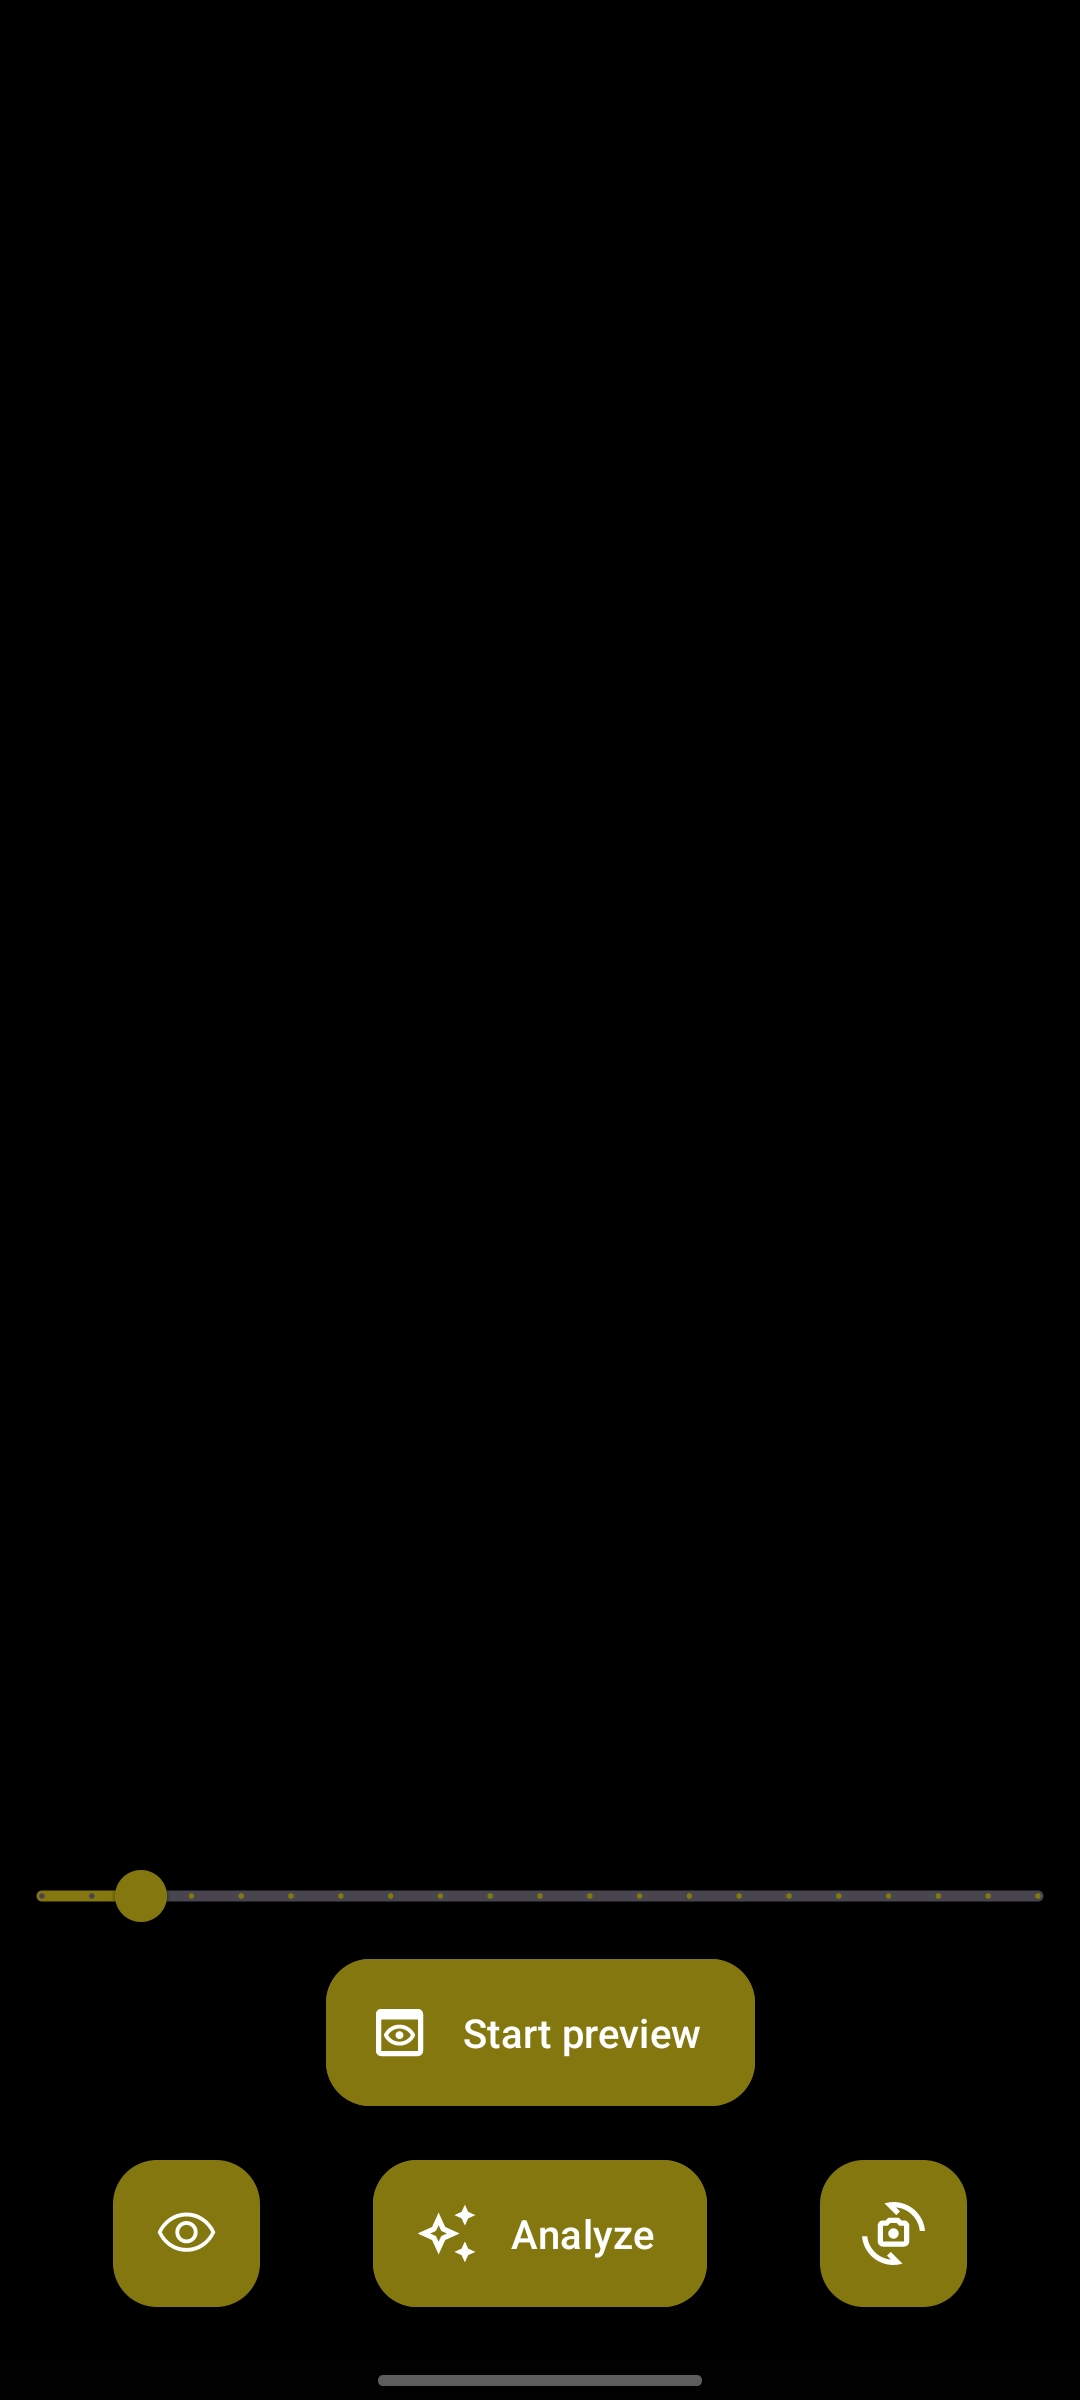
\includegraphics[scale=0.13]{ProgettoAndroid/NerdMode/Images/CameraApp_Screen_nerd_layout.jpg}
    \label{fig:nerdmodelayout}
    }
    \subfigure[Schermata Nerd mode con camera attiva]{
    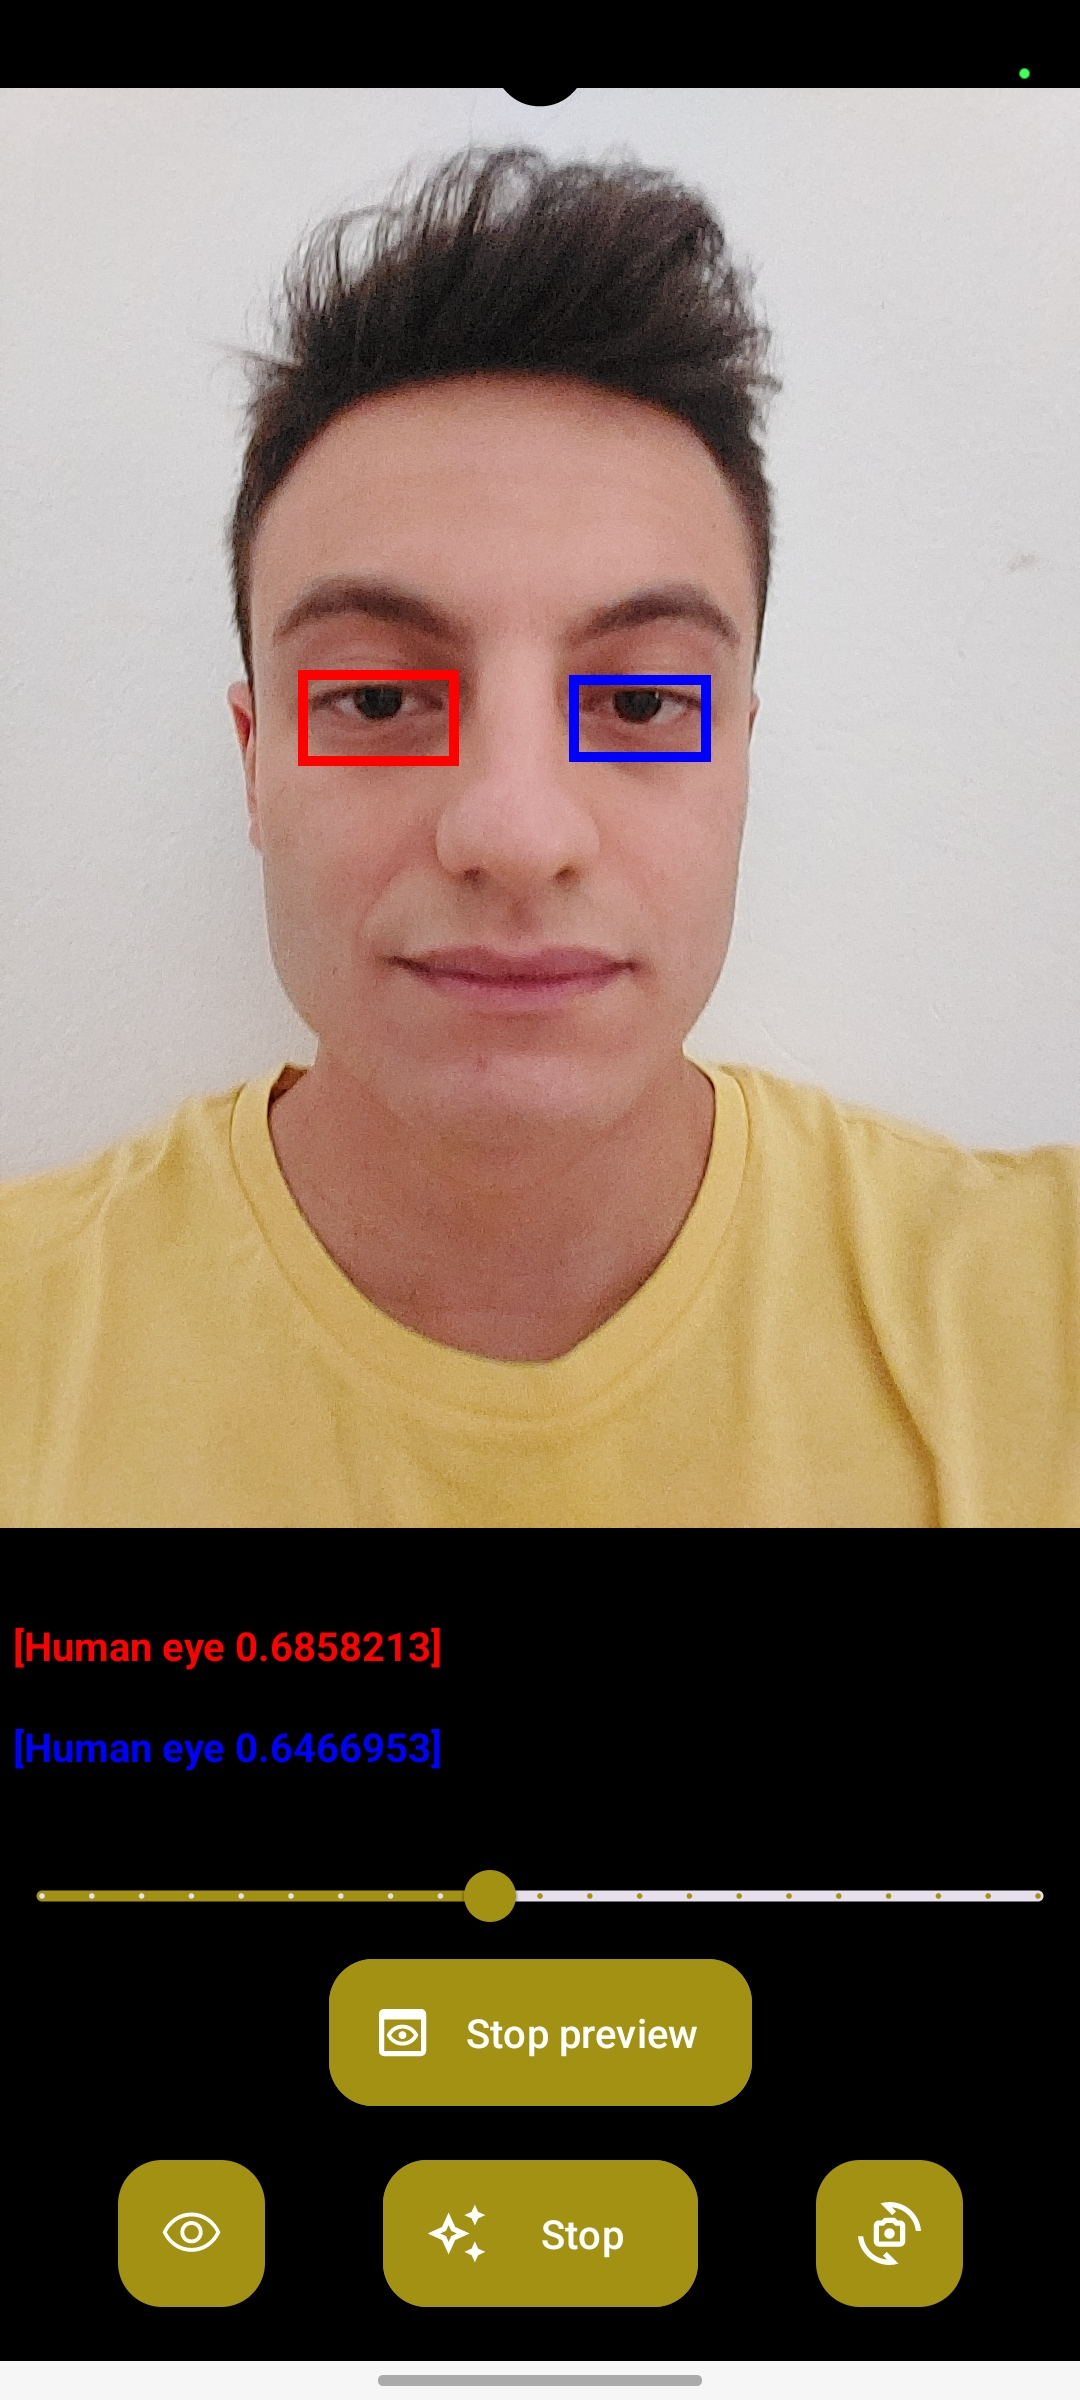
\includegraphics[scale=0.13]{ProgettoAndroid/NerdMode/Images/CameraApp_Screen_nerd.jpg}
    \label{fig:nerdmode}
    }
    \caption{Schermata Nerd}
    \label{fig:nerd}
\end{figure}

La schermata "\textit{Nerd}" è stata pensata per mostrare in modo grafico e con la maggior facilità possibile tutte le informazioni che la telecamera del dispositivo è in grado di acquisire.

Nella parte più alta dello schermo viene mostrato ciò che la telecamera acquisisce e sovrapposto l'analisi della stessa immagine tramite la rete neurale.

Per ogni occhio rilevato dalla rete neurale appare a schermo un rettangolo di colori diversi per evidenziare in che posizione è stata effettuato il tracciamento. Ulteriormente viene indicato per ogni identificazione qual è la sua accuratezza con un valore numerico decimale nell'intervallo $[0,1]$.

\subsection{Preview}
\label{sub:preview}
Il bottone "\textit{Start preview}" (vedi figura \ref{fig:nerdmodelayout}) avvia l'acquisizione dalla fotocamera del dispositivo, come fotocamera predefinita viene utilizzata quella "interna" ovvero quella rivolta verso l'utente. È possibile anche usare la fotocamera "esterna" mediante il bottone "\textit{Switch Camera}" (vedi \ref{sub:switchcamera}).

La dimensione della \textit{preview view} deve essere adattata alla dimensione del sensore della camera e quindi dell'immagine risultante. Queste dimensioni dipendono sia dal dispositivo su cui viene eseguita l'applicazione sia da quale fotocamera viene selezionata, pertanto dinamicamente l'applicazione deve adattare le dimensioni della \textit{preview view} e coerentemente il layer su cui vengono disegnati i rettangoli di tracking degli occhi. Se questa operazione non venisse effettuata o non eseguita dinamicamente la rete opererebbe comunque in maniera corretta ma la visualizzazione dei risultati risulterebbe completamente errata mostrando l'occhio in in punto dello schermo e il corrispondente rettangolo in una posizione diversa.

\subsection{Switch camera}
\label{sub:switchcamera}
Il bottone "\textit{Switch camera}" (vedi figura \ref{fig:nerdmodelayout}) permette di scegliere quale camera utilizzare per la visualizzazione e per la successiva analisi. La scelta è tra la fotocamera "interna" ovvero quella rivolta verso l'utente, lato schermo, e quella "esterna" nell'altro lato del dispositivo.

Per l'acquisizione dalla camera viene utilizzato in framework \textbf{CameraX}\cite{camerax_overview} e per costruzione, nell'attuale stato dell'arte, non permettere di scegliere, se disponibili, quale delle fotocamere esterne utilizzare, verrà dunque utilizzata in modo automatico la fotocamera esterna principale.

\subsection{Analyze}
\label{sub:analyze}
Il bottone "\textit{Analyze}" (vedi figura \ref{fig:nerdmodelayout}) è abilitato ad essere premuto sono quando è contemporaneamente abilitata la funzione "\textit{Preview}".

Alla pressione del bottone viene innescata l'analisi in tempo reale delle immagini acquisite e passate alla rete neurale per il processamento \textit{Eye-Tracking} (vedi \ref{sec:eyedetection}).

Al termine dell'analisi i risultati del tracciamento vengono mostrati a schermo su un livello grafico sovrapposto a quello di \textit{preview} della camera. Si ottiene una visualizzazione del contorno degli occhi trovati tramite rettangolo colorato e la corrispettiva accuratezza (vedi \ref{fig:nerdmode}).

È stato fondamentale gestire correttamente l'orientamento dell'immagine qualora l'utente cambi fotocamera. La fotocamera interna infatti produrrà un risultato specchiato rispetto alla visualizzazione, pertanto prima di mostrare a video i risultati ottenuti andranno orientati in base alla camera d'origine di tali dati.

Posizionato immediatamente sotto la parte di \textit{preview} è stato aggiunto uno \textit{slider} che permette di filtrare i risultati ottenuti tramite valore minimo di accuratezza.

\subsection{Attività progettuale: Riconoscimento pupilla}
\label{sub:riconoscimentopupilla}
Il bottone "\textit{Pupil-Tracking}" (vedi figura \ref{fig:nerdmodelayout}) è abilitato solo qualora sia già in esecuzione l'analisi dell'immagine.

La funzionalità di "\textit{Pupil-Tracking}" acquisisce per ogni occhio rilevato dalla fase di analisi dell'immagine un occhio e su questa porzione di immagine avvia il rilevamento della pupilla.

Al termine del processamento della rete per il riconoscimento della pupilla (vedi \ref{sec:gazedetection}) i risultati vengono mostrati a video nelle stesse modalità di quelle descritte per "\textit{Eye-Tracking}".

Qui di seguito un test effettuato direttamente su Android Studio:

\begin{figure}[htbp]
    \centering
    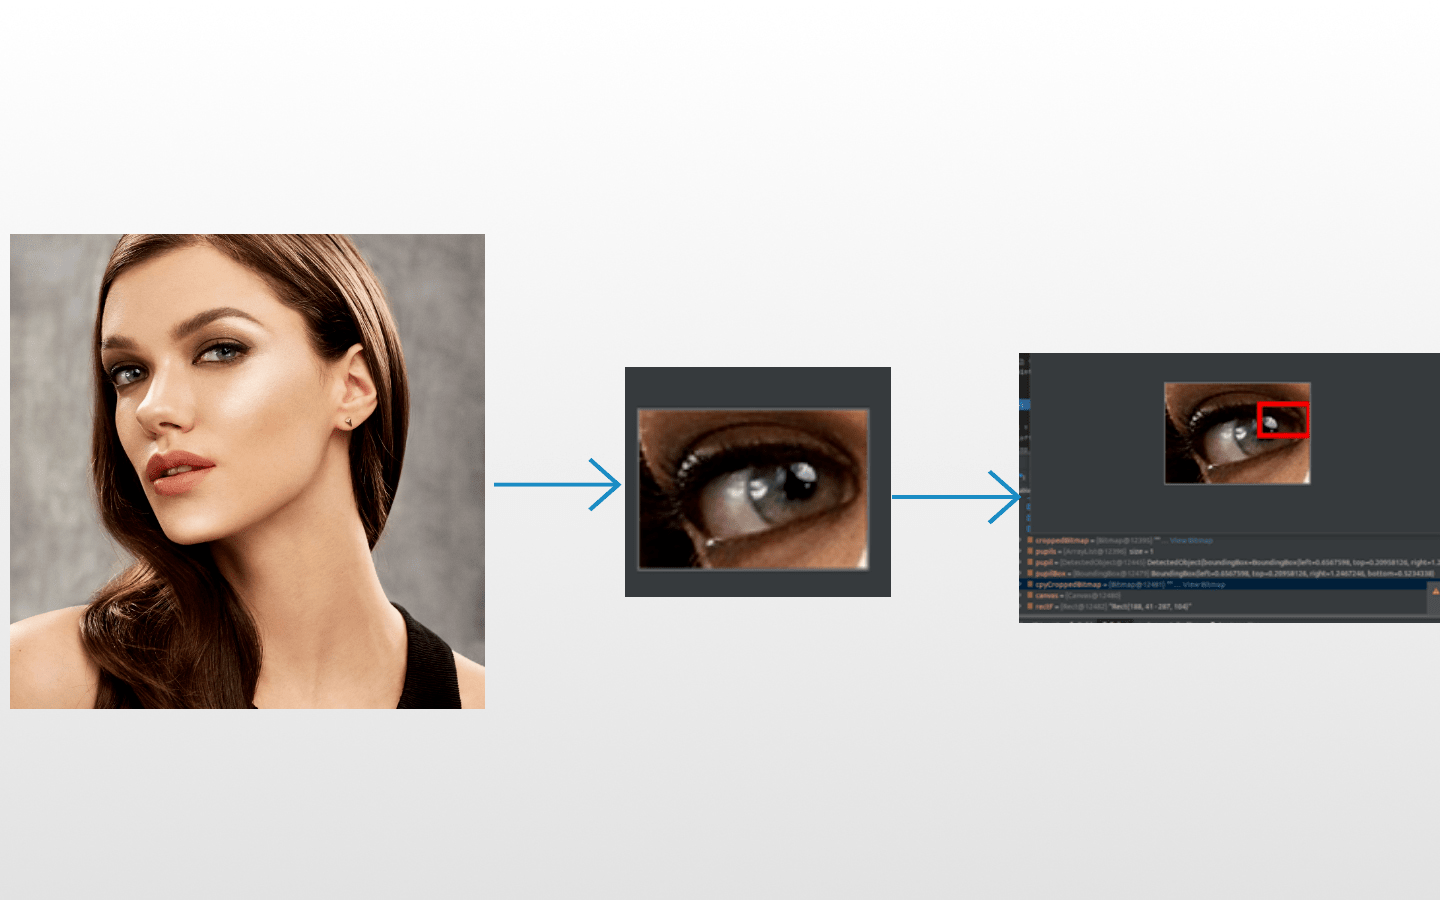
\includegraphics[scale=0.24]{ProgettoAndroid/NerdMode/RiconoscimentoPupilla/Images/gazeAndroid.png}
    \caption{Schermata Nerd mode con pupilla}
    \label{fig:nerdmodepupil}
\end{figure}